\documentclass{homework}

\title{Homework 3}
\author{Kevin Evans}
\studentid{11571810}
\date{February 3, 2021}
\setclass{Physics}{465}
\usepackage{amssymb}
\usepackage{mathtools}
\usepackage{graphicx}
\usepackage{amsthm}
\usepackage{amsmath}
\usepackage{slashed}
\usepackage{boldline}
\usepackage{physics}
\usepackage{tcolorbox}
\usepackage[inter-unit-product =\cdot]{siunitx}

\usepackage[makeroom]{cancel}
\usepackage{booktabs}
\usepackage{multirow}

\usepackage{times}
\usepackage{mhchem}
\usepackage{enumitem}
\usepackage[normalem]{ulem}
\usepackage{systeme}
\usepackage{tikz}
\usepackage{mathtools}
\usepackage{tabularx}

%\usepackage{calligra}
%\DeclareMathAlphabet{\mathcalligra}{T1}{calligra}{m}{n}
%\DeclareFontShape{T1}{calligra}{m}{n}{<->s*[2.2]callig15}{}
%\newcommand{\scriptr}{\mathcalligra{r}\,}
%\newcommand{\boldscriptr}{\pmb{\mathcalligra{r}}\,}
%\newcommand{\emf}{\mathcal{E}}

\DeclareSIUnit\eVperc{\eV\per\clight}
\DeclareSIUnit\clight{\text{\ensuremath{c}}}
\DeclareSIUnit\year{yr}

\newcommand{\fm}{\femto\meter}

\begin{document}
	\maketitle
	\begin{enumerate}
		\item \begin{enumerate}
			\item The $\delta$-function just acts as a comb, so taking the Fourier transform of the delta function results in \begin{align*}
				\mathcal{F}\left\{\delta(t)\right\} & = \int_{-\infty}^\infty \delta(t - 0) e^{i \omega t} \dd{t} \\
					& = \eval{ e^{i \omega t} }_{t=0} \\
					& = 1. \qed
			\end{align*}
	
			Next, we can use the inverse Fourier transform on $g(\omega) = 1$, \begin{align*}
				\mathcal{F}^{-1} \left\{1\right\} & = \frac{1}{2 \pi} \int_{-\infty}^\infty e^{-i \omega t} \dd{\omega} = \delta(t)
				\intertext{Since $\delta(t) \in \mathbb{R}$, the LHS must also be real and must be equal to its conjurgate,}
				\int_{-\infty}^\infty e^{i \omega t} \dd{\omega} & = 2 \pi \delta(t). \qed
			\end{align*}
			Finally, assuming the previous propositions, we can plug in a Fourier transform of an arbitrary function $f(t)$ into the inverse Fourier transform, and it should return $f(t)$, i.e. we can test \begin{align*}
				\mathcal{F}^{-1} \left\{ \mathcal{F}\left[f(t)\right] \right\} & \stackrel{?}{=} f(t). \\
				f(t) & = \frac{1}{2 \pi} \int \left\{ \int f(t') e^{i \omega t'} \dd{t'}\right\} e^{-i \omega t} \dd{\omega} \\
					& = \frac{1}{2 \pi}  \int f(t') \left\{ \underbrace{\int e^{i\omega(t' - t)} \dd{\omega}}_{2 \pi \delta} \right\} \dd{t'} && \text{reorganizing} \\
					& = \frac{1}{2 \pi} \int f(t')  2 \pi \delta(t' - t) \dd{t'} && \text{eval at $t'=t$}\\
					& = f(t). \qed
			\end{align*}
		
			\item Now, we are to show a similar proposition in $x$- and $k$-space, \begin{align*}
				\int \abs{f(x)}^2 \dd{x} & = \frac{1}{2 \pi } \int \abs{F(k)}^2 \dd{k}.
				\intertext{Starting from the RHS, we can assume complex functions and break up the square}
				\frac{1}{2 \pi} \int \abs{F(k)}^2 \dd{k} & = \frac{1}{2 \pi} \int F^*(k) F(k) \dd{k} \\
					& = \frac{1}{2 \pi} \int \dd{k} \left\{ \int f^*(x) e^{ikx} \dd{x} \right\} \left\{ \int f(x') e^{-ikx'} \dd{x'}\right\} \\
					& = \frac{1}{2 \pi} \int \dd{k} \left\{
						\iint f^*(x) f(x') 
						e^{ik(x - x')} \dd{x} \dd{x'}
					\right\}
				\intertext{Taking the $k$-integral,}
				& = \frac{1}{2 \pi} \iint f^*(x) f(x') \dd{x} \dd{x'} \int e^{ik(x-x')}\dd{k} \\
				& = \frac{1}{2 \pi} \iint f^*(x) f(x') \dd{x} \dd{x'} 2 \pi \delta(x-x') \\
				& = \int f^*(x) f(x) \dd{x} = \int \abs{f(x)}^2 \dd{x}. \qed
			\end{align*}
			
			\item Equation (5) can be rewritten in 3D as \begin{align*}
					\int \abs{f(\bvec{r})}^2 \dd[3]{\bvec{r}} & = \frac{1}{(2 \pi)^3} \int \abs{ F(\bvec{k})}^2 \dd[3]{\bvec{r}}.
				\end{align*}
				Redoing part (b), we can start with the RHS once again, then begin substituting the Fourier transform, \begin{align*}
					\frac{1}{(2 \pi)^3} \int \abs{ F(\bvec{k}) }^2 \dd[3]{\bvec{k}} & = \frac{1}{(2 \pi)^3} \int F^*(\bvec{k}) F(\bvec{k}) \dd[3]{\bvec{k}} \\
						& = \frac{1}{(2 \pi)^3} \int \dd[3]{\bvec{k} } \int \dd[3]{\bvec{r}} f^*(\bvec{r}) e^{i \bvec{k} \cdot \bvec{r}} \int \dd[3]{\bvec{r}'} f(\bvec{r}') e^{-i \bvec{k} \cdot \bvec{r}'} \\
						& = \frac{1}{(2 \pi)^3} \int \dd[3]{\bvec{k}} \iint f^*(\bvec{r}) f(\bvec{r}') e^{i\bvec{k} \cdot (\bvec{r} - \bvec{r}')} \dd[3]{\bvec{r}} \dd[3]{\bvec{r}'}.
					\intertext{Using the $\delta$-substitution given in Equation (6) and combing on $\bvec{r} = \bvec{r}'$,}
						& = \frac{1}{(2 \pi)^3} \iint f^*(\bvec{r}) f(\bvec{r}') (2 \pi)^3 \delta^3(\bvec{r} - \bvec{r}') \dd[3]{\bvec{r}} \dd[3]{\bvec{r}'} \\
						& = \int \abs{f(\bvec{r})}^2 \dd[3]{\bvec{r}}. \qed
				\end{align*}	
		
			\item Taking the Laplacian of the inverse Fourier transform, \begin{align*}
				\laplacian{f(\bvec{r})} & = \frac{1}{(2 \pi)^3} \int F(\bvec{k}) \laplacian{e^{i \bvec{k} \cdot \bvec{r}}} \dd[3]{\bvec{k}} \\
					& = \frac{1}{(2 \pi)^3} \int F(\bvec{k}) (i^2 k^2) e^{i\bvec{k} \cdot \bvec{r}} \dd[3]{\bvec{k}} \\
					& = \frac{1}{(2 \pi)^3} \int \underbrace{-k^2 F(\bvec{k})}_{FT} e^{i\bvec{k} \cdot \bvec{r}} \dd[3]{\bvec{k}}. \qed
			\end{align*}
			
			\item From the relation given in Equation (7), \begin{align*}
				\left[ \laplacian{V(\bvec{r})} \right]_{\bvec{k}} & = -k^2 \left[ V(\bvec{r})\right]_{\bvec{k}}, \\
				\implies \left[V(\bvec{r})\right]_{\bvec{k}} & = \frac{1}{k^2 \epsilon_0} \left[\rho(\bvec{r})\right]_{\bvec{k}} = \frac{e}{k^2 \epsilon_0} \left[ \delta^3(\bvec{r}) \right]_{\bvec{k}}\\ 
				& = \frac{e}{k^2 \epsilon_0}.
			\end{align*}
		\end{enumerate}
	
		\pagebreak
		
		\item We can describe the system in this figure below: \begin{center}
				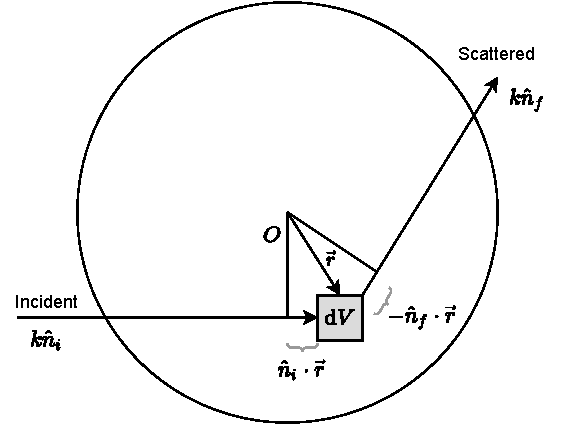
\includegraphics{formfactor.pdf}
			\end{center}
			
			The total extra phase is \begin{align*}
				e^{i \Delta \phi} & = e^{i k \uvec{n}_i \cdot \bvec{r} - i k \uvec{n}_f \cdot \bvec{r}}
				\intertext{Then, combining the $k$'s,}
				\text{Let } \bvec{\kappa} & = \uvec{k}_f - \uvec{k}_i \\
				e^{i \Delta \phi} & = e^{-i \bvec{\kappa} \cdot \bvec{r}} \\
					& = e^{-i \bvec{q} \cdot \bvec{r} / \hbar},
				\intertext{where the momentum transfer $\bvec{q}$ is given by }
				\bvec{q} & = \hbar \bvec{\kappa}.
			\end{align*}
			
		\item If we assume spherically-symmetric charge distribution, i.e. $\rho(\bvec{r}) = \rho(r)$, then the form factor is \begin{align*}
			ZeF(\bvec{\kappa}) & =\int \rho(r) e^{-i \bvec{\kappa} \cdot \bvec{r}} \dd[3]{\bvec{r}} \\
		\intertext{Using the definition of the dot product in the exponential, and rotating the axis such that all the $\theta$'s align,}
				& = \iiint \rho(r) e^{i\kappa r \cos \theta} \sin \theta \dd{\theta} \dd{\phi} r^2 \dd{r} \\
				& = 2 \pi \int_0^\infty \rho(r) r^2 \left\{ \int_0^\pi e^{-i \kappa r \cos \theta} \sin \theta \dd{\theta} \right\} \dd{r} \\
				& = 2 \pi \int_0^\infty \rho(r) r^2 \left\{ 2 \sin(\kappa r) / \kappa r \right\} \dd{r} && \text{WolframAlpha'd}\\ 
				& = \frac{ 4 \pi  }{\kappa} \int_0^\infty \rho(r) r \sin(\kappa r) \dd{r}. \qed
		\end{align*}
	
		\item From Problem 3, we can assume the charge density $\rho$ is a constant, thus the form factor is \begin{align*}
				F(\bvec{\kappa}) & = \frac{4 \pi}{Ze\kappa} \int_0^\infty \rho(r) r \sin(\kappa r) \dd{r} \\
					& = \frac{4 \pi}{Ze \kappa} \rho \int_0^a r \sin(\kappa r) \dd{r} \\
					& = \frac{4 \pi}{Ze \kappa} \rho \left[\frac{ \sin(\kappa a) - \kappa a \cos(\kappa a)}{\kappa^2} \right] \\
				\intertext{Letting $\rho = Q / V = Ze / \frac{4}{3} \pi a^3$,}
					F(\kappa) & = \frac{3}{a^3} \left[\frac{ \sin(\kappa a) - \kappa a \cos(\kappa a)}{\kappa^3} \right].
			\end{align*}
			Taking the limit as the momentum transfer goes to zero, then as $\kappa \propto q$, \begin{align*}
				\lim_{\kappa \to 0}\frac{ \sin(\kappa a) - \kappa a \cos(\kappa a)}{\kappa^3} & = \frac{a^3}{3}. && \text{WolframAlpha}
			\end{align*}
		
		\item From Problem 1(e), we found that \begin{align*}
			\left[V(\bvec{r})\right]_k & = e/k^2 \epsilon_0.
			\intertext{From the Born approximation, then}
			\mathcal{M}(\bvec{q}) & = \left[U(\bvec{r})\right]_{\bvec{k}=\bvec{q}/\hbar} \\
				& = \hbar^2 e / q^2 \epsilon_0.
			\intertext{The differential cross-section is then found directly as}
			\dv{\sigma}{\Omega} & = \left(\frac{m}{2 \pi \hbar^2}\right)^2 \left(\frac{\hbar^2 e}{q^2 \epsilon_0}\right)^2 \\
				& = \left(\frac{m}{2 \pi \hbar^2}\right)^2 \left(\frac{\hbar^2 e}{4 P^2 \sin[2](\theta / 2) \epsilon_0}\right)^2
			\intertext{Assuming classical motion, $T=p^2 / 2m \implies p^2 = 2mT$,}
			\dv{\sigma}{\Omega}	& = \left(\frac{m}{2 \pi \hbar^2}\right)^2 \left(\frac{\hbar^2 e}{8 mT  \sin[2](\theta / 2) \epsilon_0}\right)^2
			\intertext{Re-adding the forgotten $Zze$,}
			\dv{\sigma}{\Omega}	& = \left( \frac{Zze^2}{16 \pi \epsilon_0 T}\right)^2 \csc[4](\theta/2). \qed
		\end{align*}
	
	\end{enumerate}
\end{document}